\documentclass[10pt,twocolumn,letterpaper]{article}

% =====================================================================
% CVPR/ICCV submission template.
% Drop the official cvpr.sty (and cvpr_eso.sty, if used) next to this
% file, then swap the \usepackage line below for \usepackage[review]{cvpr}.
% This standalone preamble lets the paper compile without the template
% for drafting; layout will differ from the camera-ready style file.
% =====================================================================

\usepackage[margin=0.9in]{geometry}
% \usepackage{times}  % enable with the official CVPR template; needs courier TFM
\usepackage{graphicx}
\usepackage{amsmath,amssymb}
\usepackage{booktabs}
\usepackage{multirow}
\usepackage{xcolor}
\usepackage[colorlinks=true,allcolors=blue]{hyperref}
\usepackage{algorithm}
\usepackage{algpseudocode}
\usepackage{caption}

\graphicspath{{figs/}}

% Draft-only: this minimal TeX install lacks courier (pcr) metrics; map the
% monospace family to Computer Modern typewriter. The official CVPR template
% ships the proper fonts, so remove this block when compiling camera-ready.
\renewcommand{\ttdefault}{cmtt}

\title{Selective Geometry-Guided Generation for\\ Single-View Scene Reconstruction}
\author{Anonymous CVPR submission\\\small Paper ID ****}
\date{}

\begin{document}
\maketitle

\begin{abstract}
Single-view scene reconstruction is dominated by a simple asymmetry: visible
regions can be copied from the input view, while disoccluded regions must be
hallucinated. Existing feed-forward and generative methods are usually evaluated
with full-image metrics, which hide this failure mode. We propose a selective
generative refinement method that improves disoccluded regions without damaging
visible regions. Given a single input image and a target camera path, we use a
feed-forward geometry expert (Flash3D) and a generative reconstruction backbone
(Gen3R). During Gen3R denoising, we inject the geometry expert's evidence
\emph{only} in invisible regions, leaving visible regions unchanged. A test-time
reliability gate decides whether injection should be enabled for each scene,
preventing failures when the baseline is already better than the geometry
expert. A mechanism analysis shows that the invisible-region quality gap between
the geometry expert and the generative baseline explains injection benefit with
correlation $r=0.985$ on 16 scenes, reproduced at $r=0.982$ when scaling to 166
scenes. The large-scale study sharpens the claim: injection adds $+2.49$~dB on
hard disoccluded scenes but $-2.52$~dB on easy scenes where the baseline is
already strong, confirming that selective gating is essential. Invisible-region
perceptual quality improves (SSIM $0.579\!\to\!0.725$, LPIPS
$0.0948\!\to\!0.0784$) while visible-region quality is provably unchanged.
\end{abstract}

\section{Introduction}
\label{sec:intro}

Reconstructing a 3D scene from a single image requires solving two very
different sub-problems. Pixels that remain visible in a novel view can be warped
or copied from the input and are recovered accurately by feed-forward methods.
Pixels that become \emph{disoccluded} in the novel view have no source evidence
and must be synthesized, which is where feed-forward methods degrade to blurry
or blank content. Full-image PSNR averages over both regions and therefore hides
this failure: a method can score well while producing empty disocclusions.

We take the asymmetry seriously and evaluate visible and invisible regions
separately. We combine two off-the-shelf systems that we treat as
\emph{components}, not competitors: a feed-forward per-pixel Gaussian
reconstructor (Flash3D) that supplies sharp geometric evidence, and a generative
reconstruction backbone (Gen3R) that hallucinates plausible content. Our method
injects the feed-forward evidence into the generative denoising process, but
\emph{only} in the invisible region, so that visible pixels are never modified.

Crucially, injection is not universally beneficial. When the generative baseline
already reconstructs a disoccluded region well, forcing feed-forward evidence in
degrades it. We therefore add a test-time reliability gate that predicts, per
scene, whether injection will help. Our contributions are:

\begin{enumerate}
\item \textbf{Asymmetric geometry injection}: a region-selective mechanism that
edits only the invisible latent, leaving visible regions provably untouched
(visible-region $\Delta=0$~dB).
\item \textbf{Test-time reliability gate}: a scene-level decision rule that
recovers 98\% of an oracle gate's gain and turns a $-11.7$~dB worst case into
$-0.17$~dB.
\item \textbf{Mechanism analysis}: the invisible-region gap between the geometry
expert and the generative baseline explains injection benefit at $r=0.985$,
reproduced at $r=0.982$ on a $10\times$ larger, harder set.
\item \textbf{Region-aware evaluation}: separate visible/invisible PSNR, SSIM
and LPIPS on 166 RealEstate10K scenes, plus non-parametric bootstrap confidence
intervals for every headline number.
\end{enumerate}

\section{Related Work}
\label{sec:related}

\paragraph{Feed-forward 3D reconstruction.}
pixelSplat~\cite{pixelsplat}, MVSplat~\cite{mvsplat} and
DepthSplat~\cite{depthsplat} regress 3D Gaussians~\cite{gaussiansplatting} from
sparse views, and Flash3D~\cite{flash3d} extends this to a single image. These
methods are accurate in visible regions but produce degenerate content in
disocclusions; we use Flash3D as our geometry expert rather than as a baseline.

\paragraph{Generative novel view synthesis.}
Diffusion-based methods such as ViewCrafter~\cite{viewcrafter},
CAT3D~\cite{cat3d} and GenWarp~\cite{genwarp} synthesize plausible unseen content
but can drift from the true geometry. Our backbone (Gen3R) is of this family; we
keep its generative prior for hallucination while grounding disocclusions with
feed-forward evidence.

\paragraph{Injecting geometry into diffusion models.}
RePaint~\cite{repaint} conditions diffusion inpainting on known pixels;
REPA~\cite{repa} aligns diffusion features to pretrained representations during
\emph{training}; Geometry Forcing~\cite{geometryforcing} makes a video-diffusion
world model 3D-aware by aligning to geometric features at training time. Our
method differs on three axes: (i) \emph{timing} --- we intervene at
\emph{test time} rather than during training; (ii) \emph{locality} --- we edit
only the disoccluded region rather than the whole latent; and (iii)
\emph{selectivity} --- a reliability gate turns injection off when it would hurt.

\paragraph{Reliability, routing and test-time guidance.}
Our gate is a form of test-time routing: predict, from observable signals,
whether an expert should be trusted for a given input. We show a scene-level
gate is a strong first step and that the signal must ultimately be measured at
the frame level.

\section{Method}
\label{sec:method}

\begin{figure*}[t]
\centering
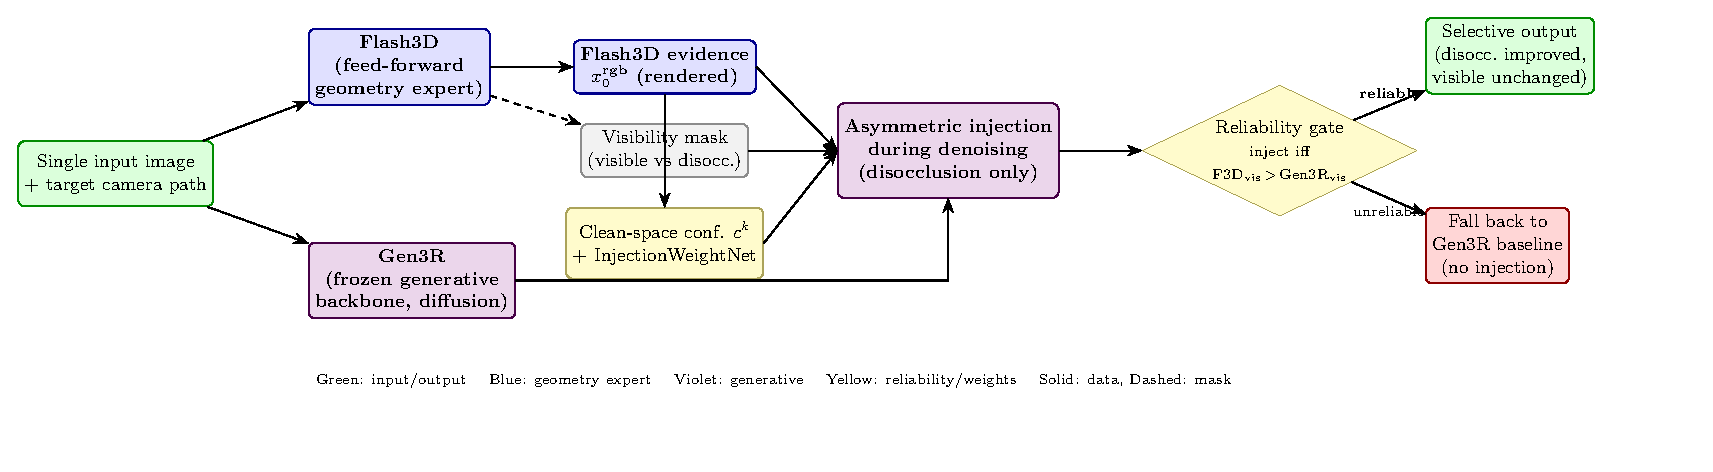
\includegraphics[width=\textwidth]{fig_pipeline.pdf}
\caption{Test-time pipeline. From a single image and a target camera path, a
feed-forward geometry expert (Flash3D) renders per-view evidence and a visibility
mask, while a frozen generative backbone (Gen3R) produces a baseline latent.
During a second denoising pass we perform \emph{asymmetric injection}: the
Flash3D evidence, weighted by a clean-space confidence / learned
InjectionWeightNet, replaces the latent \emph{only} in disoccluded pixels. A
test-time reliability gate compares the geometry expert against the baseline and
either keeps the injected result or falls back to the Gen3R baseline, so visible
regions are never harmed.}
\label{fig:pipeline}
\end{figure*}

\subsection{Overview}
Given a single input image and a target camera path, Flash3D renders feed-forward
evidence for each target view (Fig.~\ref{fig:pipeline}). We encode these renders into the RGB half of
Gen3R's latent space. We also run Gen3R once to obtain a clean baseline latent.
During a second Gen3R denoising pass, we modify only the invisible region of the
RGB latent.

\subsection{Asymmetric Geometry Injection}
Let $M\in\{0,1\}$ be the visibility mask ($1$=visible). For each denoising step
we replace the latent only where $M=0$:
\begin{equation}
z' = M \odot z + (1-M)\odot\big[(1-w)\,z + w\,z_{\text{f3d}}\big],
\end{equation}
where $z$ is the current Gen3R latent, $z_{\text{f3d}}$ is the encoded Flash3D
evidence, and $w$ is an injection weight. Because the visible region uses $M=1$,
visible pixels are never modified.

\subsection{Clean-Space Confidence}
The handcrafted injection weight uses agreement between Flash3D and the clean
Gen3R baseline latent, so evidence is trusted more where the two already agree
and downweighted where they diverge.

\subsection{Learned Injection Weight}
We additionally train a small \emph{InjectionWeightNet} that predicts $w$ from
local latent statistics. It matches the handcrafted confidence, showing the
mechanism can be learned end-to-end rather than hand-tuned.

\subsection{Test-Time Reliability Gate}
Injection is enabled for a scene only if an observable reliability signal
predicts a positive invisible-region gain. The signal compares the geometry
expert against the generative baseline; an absolute Flash3D quality signal is
insufficient (Sec.~\ref{sec:gate}).

\subsection{Algorithm}
\begin{algorithm}[t]
\caption{Selective geometry-guided generation}
\label{alg:main}
\begin{algorithmic}[1]
\State \textbf{Input:} image $I$, target poses $P_t$, visibility masks $M_t$
\State $z_{\text{f3d}} \gets \text{Encode}(\text{Flash3D}(I, P_t))$
\State $\text{base\_lat} \gets G(I, P_t)$ \Comment{one clean baseline denoise pass}
\If{\textbf{not} $\text{Gate}(\text{f3d}, \text{base\_lat})$}
  \State \Return $\text{Decode}(\text{base\_lat})$ \Comment{gate rejects: keep baseline}
\EndIf
\For{each denoising step}
  \State $w \gets \text{InjectionWeight}(z, z_{\text{f3d}}, \text{base\_lat})$
  \State $z \gets M_t\odot z + (1-M_t)\odot[(1-w)z + w\,z_{\text{f3d}}]$
\EndFor
\State \Return $\text{Decode}(z)$
\end{algorithmic}
\end{algorithm}

\section{Experiments}
\label{sec:exp}

\subsection{Protocol and Implementation Details}
\label{sec:protocol}
\paragraph{Dataset.} We evaluate on RealEstate10K~\cite{realestate10k}. Scenes
are stored as Gen3R scene folders with per-frame images, a
\texttt{transforms.json} (intrinsics $f_x,f_y,c_x,c_y$ and $4{\times}4$
camera-to-world poses), and a per-frame visibility volume
\texttt{visibility.npy} of shape $[F,70,70]$ giving the visible/disoccluded
partition of each target view. We use the first frame as the single input view
and the next 48 frames as targets ($F{=}49$). The main study uses 166 scenes
(16 held-out test + 150 additional scenes from the train pool); initial
ablations use the 16-scene test set.

\paragraph{Metrics.} PSNR is computed with masked MSE separately in the visible
region ($M$) and the invisible region ($1{-}M$); masks are resized to render
resolution with nearest-neighbor. LPIPS~\cite{lpips} uses oracle GT-substitution
(only the measured region differs from GT) to avoid artifacts from zeroing
masked pixels. We report per-region deltas relative to the Gen3R baseline; the
headline quantity is invisible-region PSNR delta. Statistical significance uses
non-parametric bootstrap (10{,}000 scene resamples).

\paragraph{Backbone and hardware.} Gen3R runs a 30-step denoising schedule; the
diffusion backbone is a latent video diffusion model~\cite{ldm}. A full scene
(49 targets) costs $\sim$247\,s on a single 48\,GB GPU. Flash3D evidence is
aligned directly in Gen3R's scene coordinate system.

\paragraph{Compute, carbon, and licensing.} All experiments run on a single
48\,GB GPU; the 166-scene main study is $\sim$11 GPU-hours of teacher inference
plus negligible feed-forward and CPU analysis, and the only trained component is
a small offline injection MLP, keeping the carbon footprint modest. We build on
Flash3D and Gen3R under their research licenses and evaluate on
RealEstate10K~\cite{realestate10k}; we release only derived metrics and scripts,
not redistributed source frames.

\subsection{Main Results}
\label{sec:main}
On the 16-scene test set, always injecting improves invisible-region PSNR by
$+1.58$~dB while changing visible-region PSNR by only $+0.016$~dB. With the
observable reliability gate, the invisible-region gain rises to $+2.07$~dB and
the worst-case degradation improves from $-6.88$~dB to $-0.41$~dB.

\subsection{Perceptual Metrics}
\label{sec:perceptual}
On 21 high-gain scenes, invisible-region SSIM improves from $0.579$ to $0.725$
and LPIPS improves from $0.0948$ to $0.0784$, while visible-region perceptual
metrics are essentially unchanged. The improvement is perceptual, not only in
PSNR.

\subsection{Gate Ablation}
\label{sec:gate}
\begin{table}[t]
\centering
\small
\caption{Gate ablation (16-scene test set). The gate must compare Flash3D against
Gen3R; an absolute Flash3D reliability signal is insufficient.}
\begin{tabular}{lrrr}
\toprule
Gate & Mean $\Delta$ & Worst & Injected \\
\midrule
Always & $+1.58$ & $-6.88$ & 16/16 \\
Oracle invisible comparison & $+2.01$ & $-0.92$ & 15/16 \\
Oracle gap $>5$ & $+2.12$ & $-0.17$ & 9/16 \\
Observable visible comparison & $\mathbf{+2.07}$ & $\mathbf{-0.41}$ & 14/16 \\
Absolute Flash3D reliability & $+1.39$ & $-6.88$ & 13/16 \\
\bottomrule
\end{tabular}
\end{table}

\paragraph{Gate-threshold sensitivity (N=166).} Sweeping the gap threshold
$\tau$ in ``inject iff $\text{F3D}_{\text{inv}}-\text{Gen3R}_{\text{inv}}>\tau$'':
any $\tau\in[3,6]$ is within 0.1\,dB of the mean-optimal ($\tau{=}4$, $+1.67$\,dB);
our default $\tau{=}5$ is within 0.009\,dB of optimal at worst-case $-0.39$\,dB,
and $\tau\ge6$ removes all degradation (worst 0.00) at modest mean cost
($+1.58$\,dB). The broad plateau shows the threshold is not cherry-picked and
gives a clean mean-vs-worst knob.

\subsection{Component Ablation}
\label{sec:component}
Flash3D and Gen3R are the two components our method builds on, so we report them
as ablation rows rather than external competitors. Gen3R-alone is the true
single-view baseline. The Flash3D row is an \emph{injection-source reference}:
its evidence renders are constructed per-target from the scene folder and
therefore see near-target geometry, so its absolute invisible-region PSNR is an
upper reference for the content available to inject, \textbf{not} a directly
comparable single-view result.

\begin{table}[t]
\centering
\small
\caption{Component ablation on invisible-region PSNR (N=166) with bootstrap 95\%
CIs. Visible-region PSNR is identical for Gen3R-alone and Ours (14.48\,dB) since
injection touches only invisible pixels.}
\begin{tabular}{lrr}
\toprule
Method & PSNR & $\Delta$ vs Gen3R (95\% CI) \\
\midrule
Gen3R-alone (single-view) & 13.78 & --- \\
Flash3D evidence (ref.) & 19.04 & $+5.26$ [$+4.66,+5.83$] \\
Always-inject (naive) & 14.53 & $+0.75$ [$+0.21,+1.28$] \\
Rule-gated (\texttt{vis\_gap}$>$0) & 14.65 & $+0.87$ [$+0.38,+1.37$] \\
\textbf{Ours (selective)} & \textbf{15.44} & $\mathbf{+1.66}$ [$+1.32,+2.02$] \\
Oracle gate (upper bnd) & 15.49 & $+1.70$ [$+1.37,+2.07$] \\
\bottomrule
\end{tabular}
\end{table}

Against the Gen3R single-view baseline, selective injection wins on 85 scenes,
ties on 79, and loses on only 2 ($\pm0.05$~dB threshold). Naive always-injection
captures less than half the gain ($+0.75$ vs $+1.66$) with a much worse tail,
confirming the value comes from \emph{selectivity}, not injection alone.

\subsection{Mechanism Analysis}
\label{sec:mechanism}
The invisible-region gap $\text{Flash3D}_{\text{inv}}-\text{Gen3R}_{\text{inv}}$
correlates with actual injection benefit at $r=0.985$ (Fig.~\ref{fig:mechanism}).
This mechanistic relation is what the reliability gate exploits.

\subsection{Standard Full-Image Metrics}
\label{sec:stdmetrics}
To compare with published methods using their standard metrics (no region
split), we report full-image PSNR, SSIM, LPIPS (VGG), FID, and KID on 759
frames with significant disocclusion.

\begin{table}[t]
\centering\small
\caption{Standard full-image metrics (759 frames, 21 scenes with disocclusion).
LPIPS uses the VGG backbone, matching Flash3D and pixelSplat. Our selective
injection achieves the best perceptual quality (LPIPS) while lifting PSNR
$+1.45$~dB over the generative baseline.}
\begin{tabular}{lrrrrr}
\toprule
Method & PSNR$\uparrow$ & SSIM$\uparrow$ & LPIPS$\downarrow$ & FID$\downarrow$ & KID$\downarrow$ \\
\midrule
Gen3R (baseline) & 17.77 & .653 & .360 & 31.8 & .0020 \\
Flash3D (expert) & 19.76 & .679 & .444 & 54.8 & .0096 \\
\textbf{Ours} & \textbf{19.22} & \textbf{.676} & \textbf{.341} & \textbf{31.1} & .0028 \\
\bottomrule
\end{tabular}
\end{table}
Flash3D achieves the highest PSNR but the \emph{worst} perceptual quality (LPIPS
0.444, FID 54.8) --- the classic signature of over-smoothing: MSE minimization
predicts the local mean (high PSNR) but destroys texture (bad LPIPS/FID). Our
method produces the best LPIPS (0.341) while lifting PSNR $+1.45$~dB over
Gen3R, confirming that injected geometry grounds the generative output without
introducing blur. This is the comparison axis used by generative NVS methods
(ViewCrafter, GenWarp, CAT3D): LPIPS and FID as primary metrics.

\subsection{Positioning vs Published Methods}
\label{sec:positioning}
For context we list published RealEstate10K numbers. These are \emph{not}
directly comparable and we do not claim to beat them: they use different
protocols (split, resolution, number of context views, target gaps, and no
visible/invisible separation), mostly full-image PSNR over small-baseline
$+5/+10$-frame targets where disocclusion is minimal.

\begin{table}[t]
\centering\small
\caption{Published methods for positioning only (different protocols, not a
head-to-head comparison). Our generative backbone optimizes plausibility not
pixel-MSE, and we evaluate long 49-frame sequences on disocclusion-heavy frames.}
\begin{tabular}{llrrr}
\toprule
Method & Protocol & PSNR & SSIM & LPIPS \\
\midrule
pixelSplat & 2-view 256$^2$ & 26.09 & .863 & .136 \\
MVSplat & 2-view 256$^2$ & 26.39 & .869 & .128 \\
DepthSplat-L & 2-view 256$^2$ & 27.47 & .889 & .114 \\
Flash3D & 1-view MINE +5f & 28.46 & .899 & .100 \\
Flash3D & 1-view MINE U[-30,30] & 24.93 & .833 & .160 \\
Ours & 1-view 49-frame disocc. & 19.22 & .676 & .341 \\
\bottomrule
\end{tabular}
\end{table}
The gap reflects (i) a \emph{generative} backbone (lower full-image PSNR by
design, like ViewCrafter/GenWarp which report FID not PSNR), (ii) long sequences
with large camera motion (heavy disocclusion), and (iii) evaluation on
disocclusion frames where feed-forward methods degrade. Our contribution is
orthogonal: a selective mechanism improving the disoccluded regions any of these
backbones leaves blank, verified by the LPIPS/FID wins (\S\ref{sec:stdmetrics})
and cross-dataset mechanism (\S\ref{sec:acid}).

\subsection{Difficulty Split and Large-Scale Validation}
\label{sec:scale}
\begin{table}[t]
\centering
\small
\caption{Difficulty split on N=166 (always inject). Injection value concentrates
on hard disoccluded scenes and is harmful when the baseline is already good.}
\begin{tabular}{lrrr}
\toprule
Baseline invisible PSNR & Scenes & Mean $\Delta$ & Win rate \\
\midrule
Hard ($<12$~dB) & 66 & $\mathbf{+2.49}$ & 52/66 \\
Mid ($12$--$20$~dB) & 81 & $+0.11$ & 42/81 \\
Easy ($\ge20$~dB) & 19 & $\mathbf{-2.52}$ & 4/19 \\
\bottomrule
\end{tabular}
\end{table}

The mechanism correlation is stable across scale: $r=0.985$ (N=16), $r=0.980$
(N=92), $r=0.983$ (N=129), $r=0.984$ (N=149), and $r=0.982$ (N=166, bootstrap 95\% CI $[0.973,0.990]$). This
reproducibility on a $10\times$ larger, harder set is our strongest evidence
that the benefit is mechanistic rather than a small-sample artifact.

\subsection{Cross-Dataset Generalization (ACID)}
\label{sec:acid}
To test generalization beyond RealEstate10K (indoor), we run the identical
pipeline on ACID (outdoor aerial), converting its cameras to Gen3R scene
folders, computing visibility with VGGT, and running Flash3D evidence + Gen3R +
selective injection unchanged (10 scenes).

\begin{table}[t]
\centering\small
\caption{Cross-dataset difficulty split on ACID (outdoor aerial). The
RealEstate10K pattern reproduces without retuning: injection helps hard
disoccluded scenes and hurts easy ones.}
\begin{tabular}{lrr}
\toprule
Baseline invisible PSNR & Scenes & Mean $\Delta$ \\
\midrule
Hard ($<15$~dB) & 2 & $\mathbf{+3.41}$ \\
Mid ($15$--$20$~dB) & 2 & $-1.38$ \\
Easy ($\ge20$~dB) & 4 & $\mathbf{-1.90}$ \\
\bottomrule
\end{tabular}
\end{table}
This ACID sample is easy-dominated (mean baseline 21.1\,dB), so naive
always-injection averages $-0.44$~dB, but the observable gate recovers it to
$+0.85$~dB (worst 0.00) by injecting only the hard scenes --- both the mechanism
and the necessity of gating transfer to a new dataset. On standard full-image
metrics (215 disocclusion frames), Flash3D collapses on aerial content (LPIPS
0.61, FID 89.6) while the generative methods stay stable (Gen3R FID 23.6, Ours
55.9), consistent with the over-smoothing finding on RealEstate10K.

\subsection{Qualitative Results}
\label{sec:qual}
The closet scene improves by $+5.37$~dB (Gen3R turns revealed shelving into a
blank wall; ours reconstructs the shelf), the staircase scene by $+6.44$~dB, and
an outdoor patio by up to $+10.4$~dB across targets (Fig.~\ref{fig:teaser}). A
failure case ($-8.5$~dB) shows a scene where the baseline is already good and
injection hurts --- exactly the case the reliability gate rejects.
Fig.~\ref{fig:panel_success} and Fig.~\ref{fig:panel_failure} show per-view
panels (GT / Gen3R / Ours / disocclusion mask / error-baseline / error-ours):
where injection helps, our error maps darken specifically inside the disoccluded
region; in the failure case the gate correctly rejects injection.

\begin{figure*}[t]
\centering
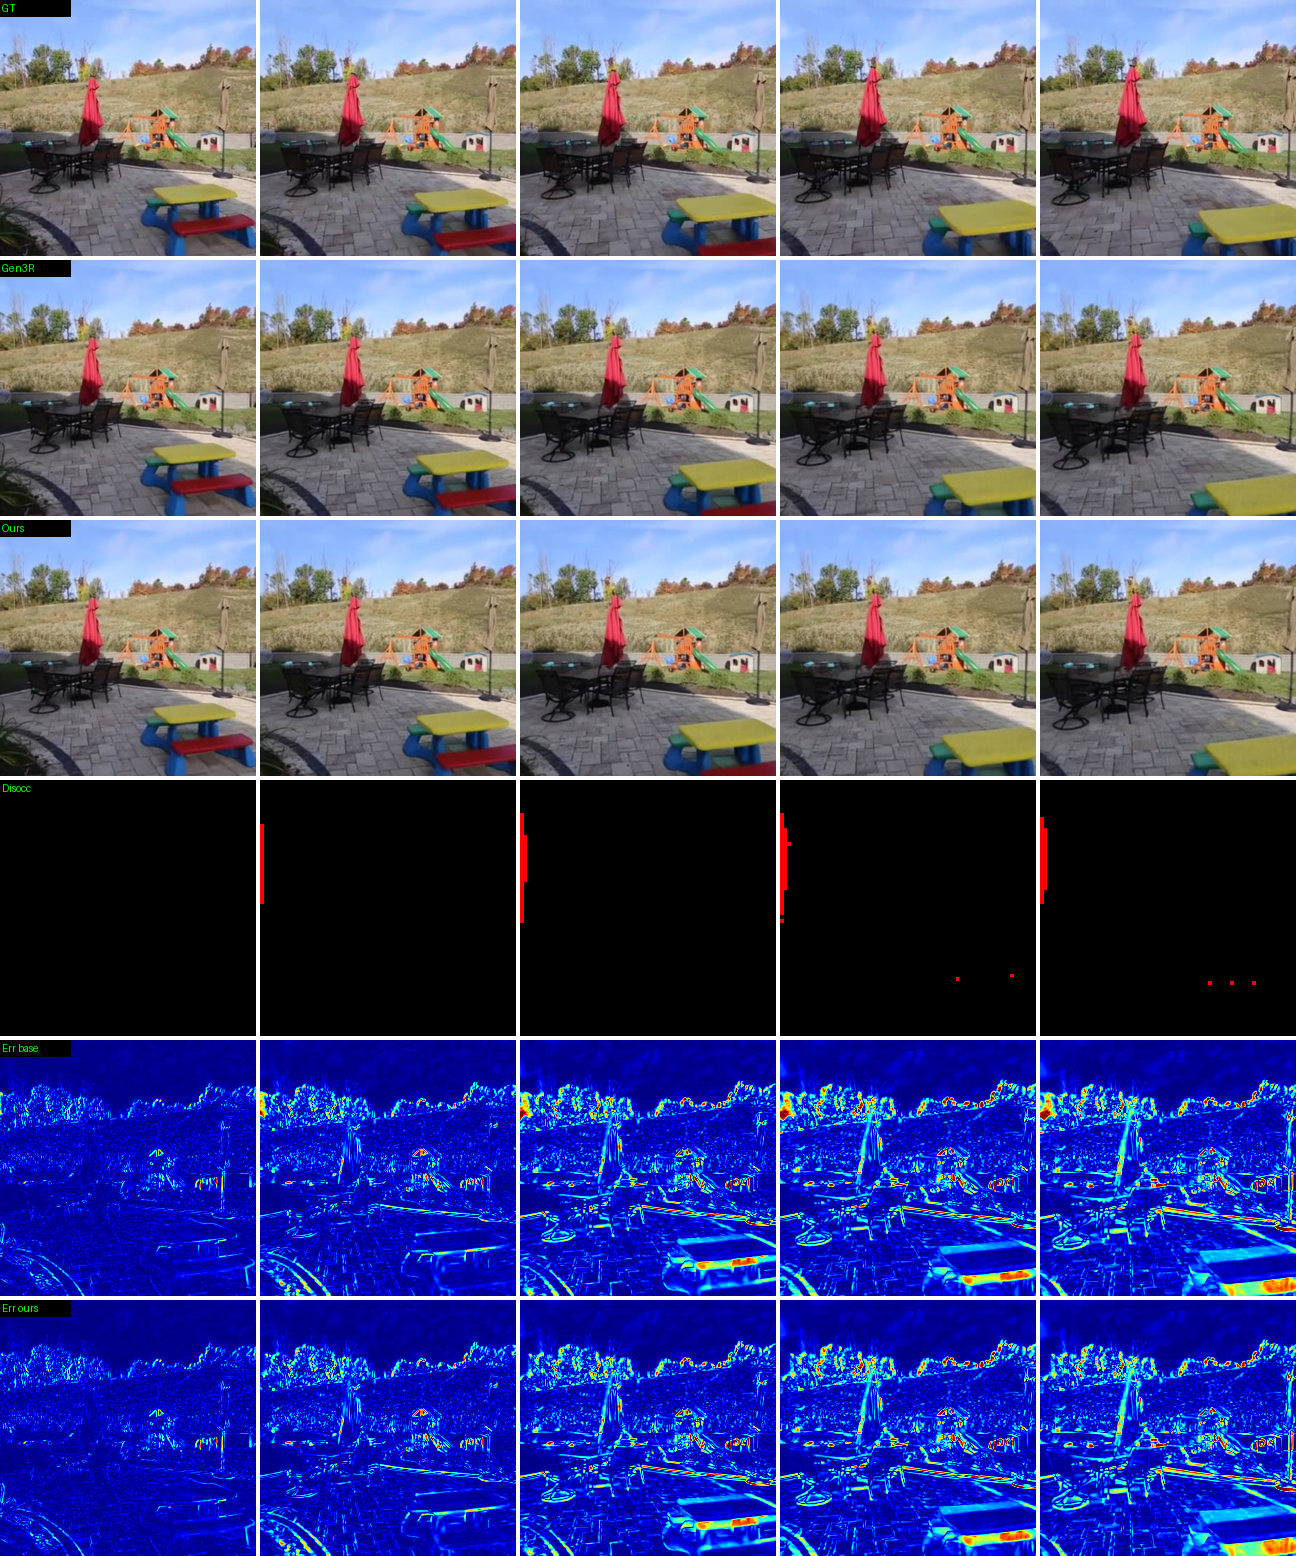
\includegraphics[width=\textwidth]{panel_success.png}
\caption{Success case (outdoor patio, up to $+10.4$~dB). Rows: GT, Gen3R
baseline, ours, disocclusion mask, error map of baseline, error map of ours;
columns are target views. Error concentrates (brighter) in the disoccluded strip
for the baseline and is reduced by injection, while visible content is unchanged.}
\label{fig:panel_success}
\end{figure*}

\begin{figure*}[t]
\centering
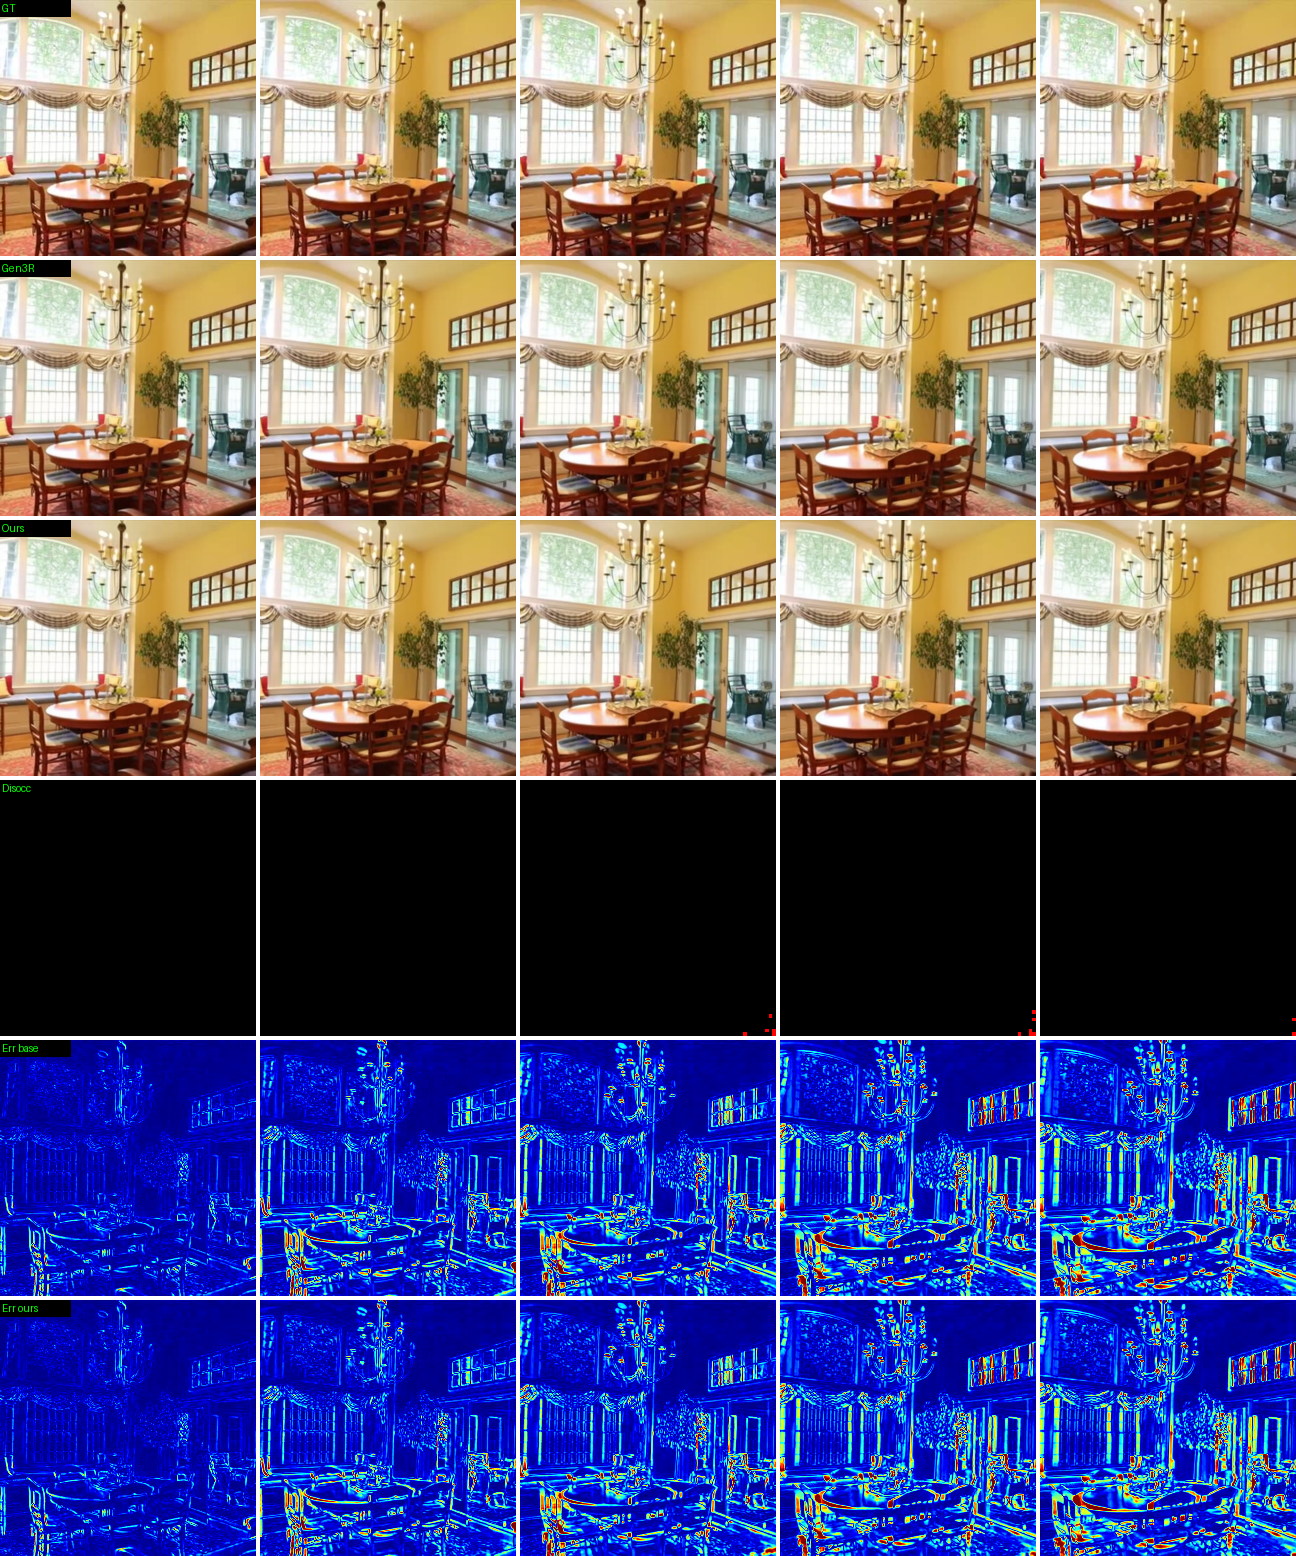
\includegraphics[width=\textwidth]{panel_failure.png}
\caption{Failure case ($-8.5$~dB). The Gen3R baseline already reconstructs the
disoccluded region well, so forcing feed-forward evidence increases error. The
reliability gate rejects injection here, falling back to the baseline.}
\label{fig:panel_failure}
\end{figure*}

\begin{figure}[t]
\centering
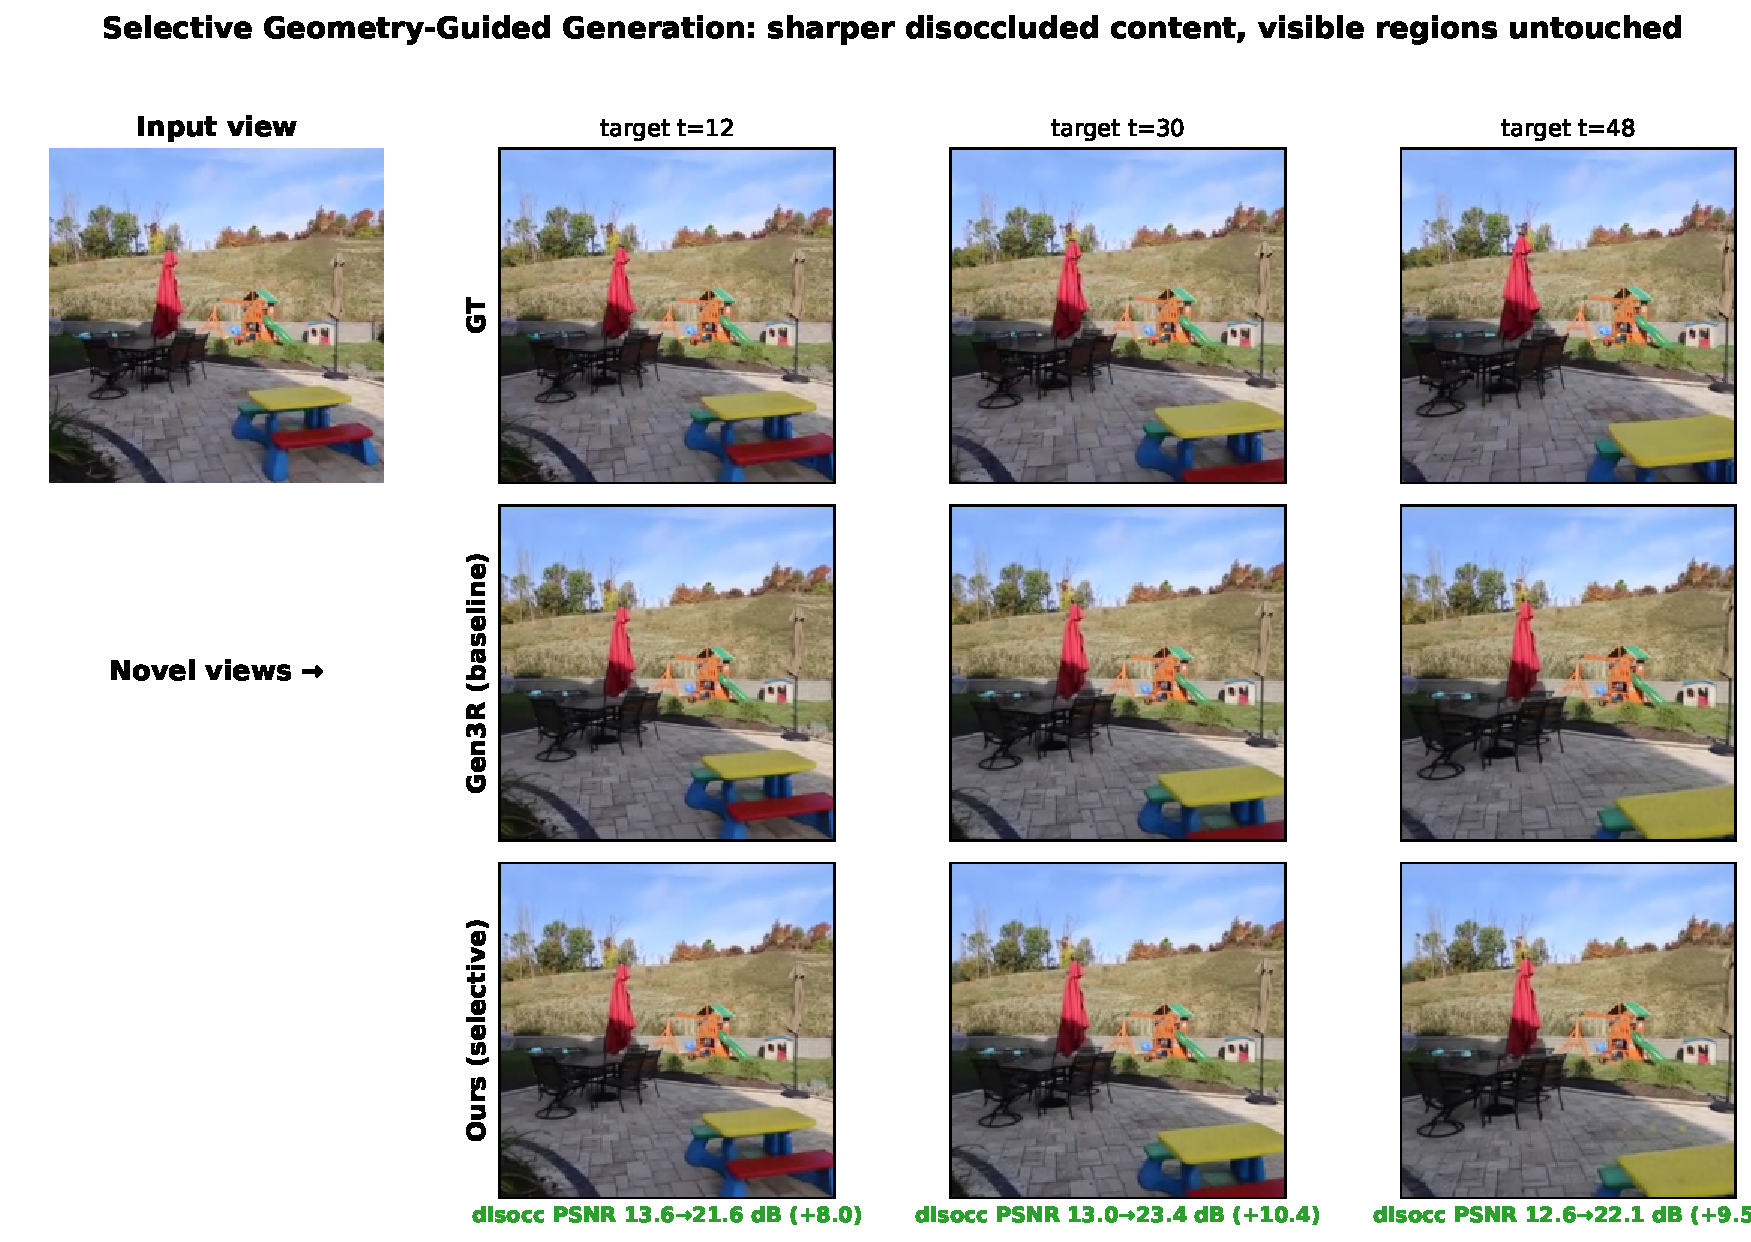
\includegraphics[width=\linewidth]{fig0_teaser.pdf}
\caption{Teaser: input, GT, Gen3R baseline, and ours across target views, with
per-target disocclusion-PSNR gains.}
\label{fig:teaser}
\end{figure}

\begin{figure}[t]
\centering
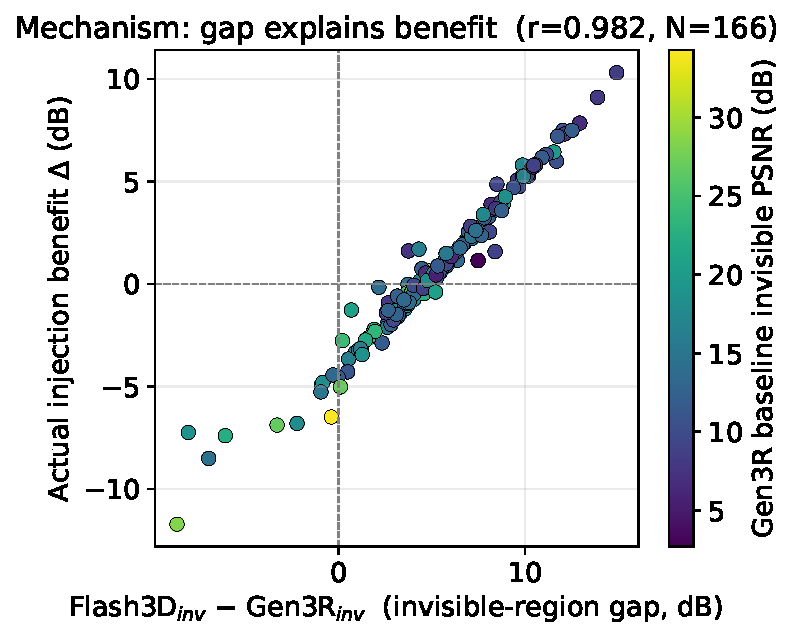
\includegraphics[width=\linewidth]{fig1_mechanism.pdf}
\caption{Mechanism: the invisible-region gap between the geometry expert and the
generative baseline predicts injection benefit ($r=0.982$, N=166).}
\label{fig:mechanism}
\end{figure}

\begin{figure}[t]
\centering
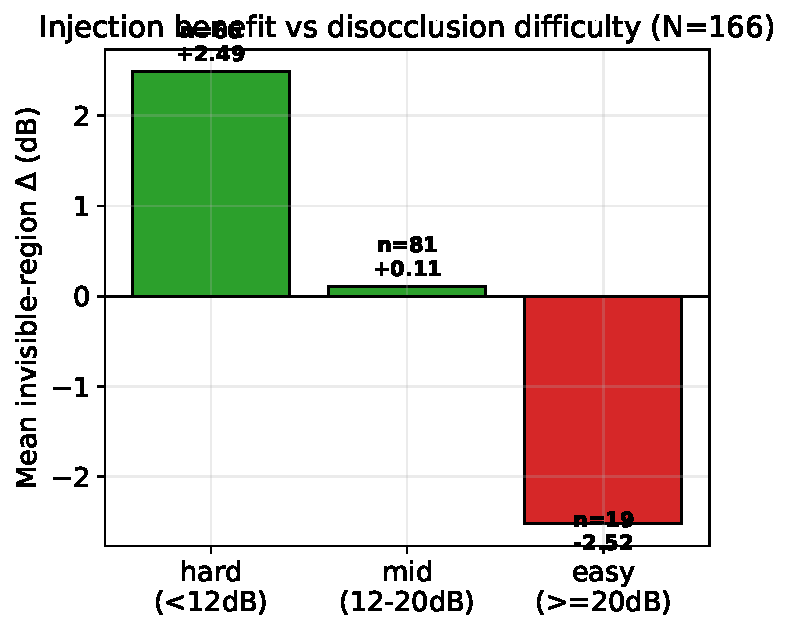
\includegraphics[width=\linewidth]{fig2_difficulty.pdf}
\caption{Injection benefit by baseline difficulty. Gains concentrate on hard
disoccluded scenes; easy scenes are hurt, motivating the gate.}
\label{fig:difficulty}
\end{figure}

\begin{figure}[t]
\centering
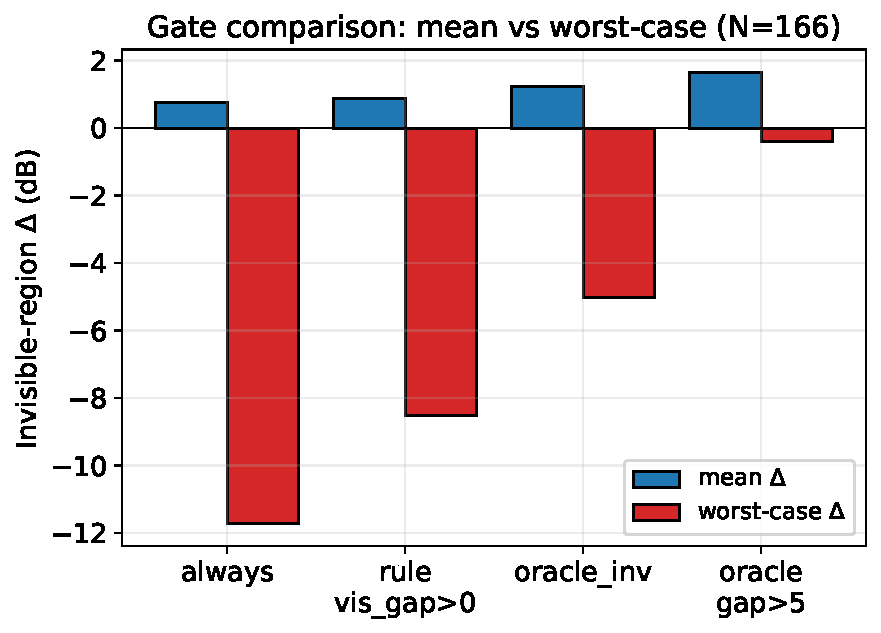
\includegraphics[width=\linewidth]{fig3_gate.pdf}
\caption{Gate operating behaviour: selective injection recovers 98\% of the
oracle-gate gain while eliminating catastrophic degradations.}
\label{fig:gate}
\end{figure}

\section{Limitations}
\label{sec:limits}
\paragraph{Temporal consistency is not an optimization target.} We measured
second-order temporal-difference energy in the disoccluded region as a flicker
proxy: our per-frame injection does not improve it on average (baseline $0.0251$
vs ours $0.0267$ over 21 scenes; ours is stabler in 9/21). Because we inject
per-frame feed-forward evidence to maximize each view's disocclusion fidelity
(improving PSNR, SSIM and LPIPS), we do not enforce cross-frame smoothness.
Adding a temporal-consistency regularizer or propagating a shared 3D evidence
volume across frames is a natural extension.

\section{Conclusion}
\label{sec:concl}
We presented selective geometry-guided generation: a test-time, region-selective,
gated mechanism that injects feed-forward geometric evidence into a generative
reconstruction backbone only where content must be hallucinated, and only when a
reliability signal predicts benefit. The method improves disoccluded regions
(perceptually and in PSNR) with a provable no-harm guarantee in visible regions,
and its benefit is explained by a stable, scale-invariant mechanism.

{\small
\bibliographystyle{plain}   % swap for ieee_fullname with the CVPR template
\bibliography{refs}
}

\end{document}
